\documentclass [12pt,oneside] {article}

% Codificação dos caracteres da entrada (use ISO no Windows e UTF no Linux)
%\usepackage[isolatin]{inputenc}  % arquivos LaTeX em ISO-8859-1
\usepackage[utf8]{inputenc}     % arquivos LaTeX em Unicode

% packages usados na construção deste documento
\usepackage [T1]{fontenc}        % caracteres acentuados corretos na saida
\usepackage {times}              % Fontes Times
\usepackage [portuguese]{babel}      % texto em portugues
\usepackage {indentfirst}        % indentar primeiro paragrafo
\usepackage {epsfig}             % inclusao de figuras em formato EPS
\usepackage[hidelinks]{hyperref}
\usepackage{float}				 % para imagens

% usar papel no formato A4 com margens 30,30,25,25 mm^M
\usepackage[a4paper,top=30mm,bottom=30mm,left=25mm,right=25mm]{geometry}

% relaxar o espaçamento entre caracteres
% \sloppy

% O espaçamento entre linhas deve ser 1.5
% \renewcommand{\baselinestretch}{1.5}

% indentação dos parágrafos é 15mm
\setlength{\parindent}{15mm}

% pacote sugerido para formata��o de c�digo-fonte
\usepackage{listings}
\lstset{language=c}
\lstset{inputencoding=latin1,extendedchars=true}
\lstset{basicstyle=\small,commentstyle=\textit,stringstyle=\ttfamily}
\lstset{showspaces=false,showtabs=false,showstringspaces=false}
\lstset{numbers=left,stepnumber=5,numberstyle=\tiny}
\lstset{columns=flexible,mathescape=true}
\lstset{frame=single}

% pacote sugerido para formatação de algoritmos
\usepackage{algorithm,algorithmic}
\floatname{algorithm}{Algoritmo}
\renewcommand{\algorithmiccomment}[1]{~~~// #1}
 % incluir pacotes e configurações

%=====================================================

\begin {document}

\title {Relatório sobre \emph{contexts.c}}
\author {Waine Junior \and Giovanni Forastieri}
\date {Agosto de 2019}
\maketitle

%=====================================================

\section{Introdução}
Este relatório tem como objetivo explicar a execução do código presente no arquivo \emph{contexts.c}. Primeiro descrevendo os objetivos e parâmetros das funções referentes a contextos presentes nele. Depois a estrutura de dado utilizada. Por fim o que cada linha de código que manipulam contextos fazem. Além disso, é apresentado o diagrama de tempo da execução do código.

\section{Funções}

O código utiliza funções padrão POSIX para manipulação de contexto. São elas:
\begin{itemize}
	\item \texttt{getcontext(\&a)}: tem como objetivo obter o atual contexto do programa e gravá-lo na variável \texttt{a}, a qual é do tipo \texttt{ucontext\_t}, estrutura explicada na seção \ref{sec:estr_dados}.
	\item \texttt{setcontext(\&a)}: tem como objetivo alterar o contexto atual, restaurando aquele apontado pela variável \texttt{a}.
	\item \texttt{swapcontext(\&a,\&b)}: tem como objetivo trocar o contexto, salvando o atual em \texttt{a} e restaurando aquele em \texttt{b}. É equivalente à chamada de \texttt{getcontext(\&a);} seguida de
	\texttt{setcontext(\&b);}.
	\item \texttt{makecontext(\&a, ...)}: tem como objetivo alterar o contexto salvo em \texttt{a}, mais especificamente a "função chamada" por esse e os argumentos passados para essa.
\end{itemize}

\section{Estruturas de dados}\label{sec:estr_dados}

Para o armazenamento das propriedades do contexto, é utilizada um estrutura de dado presente no arquivo \emph{ucontext.h}, denominada \texttt{ucontext\_t}. O significado dos campos da estrutura utilizados no código é:

\begin{itemize}
	\item \texttt{void* uc\_stack.ss\_sp}: \emph{stack pointer} da pilha de sinal (\emph{signal stack}).
	\item \texttt{size\_t uc\_stack.ss\_size}: tamanho, em bytes, da pilha de sinal. Deve ser definido como o tamanho alocado para a pilha. O arquivo \emph{signal.h} define um valor padrão para ser utilizados: \texttt{SIGSTKSZ}, tamanho canônico.
	\item \texttt{int uc\_stack.ss\_flags}: operador ou lógico entre as \emph{flags} \texttt{SS\_DISABLE } e\\ \texttt{SS\_ONSTACK}. A primeira diz para o sistema se a pilha de sinal não deve ser utilizada. A segunda é uma variável setada pelo sistema que diz se a pilha está em uso atualmente. Caso não esteja em uso, os sinais devem ser entregues à pilha do usuário normal 
	\item \texttt{ucontext\_t.uc\_link}: aponta para o contexto que será resumido após o fim da execução do contexto da estrutura.
\end{itemize}

A pilha de sinal (\emph{signal stack}) é utilizada para definir o tratamento dos sinais gerados durante a execução de um programa, por meio da função \texttt{signal()} ou \texttt{sigaction()}. O levantamento de um sinal pode ser feita por meio das chamadas \texttt{kill()} e \texttt{raise()}. Os tipos padrão de sinais que podem ser gerados são definidos no arquivo \emph{signal.h} \cite{ManualGNU2019}.

\section{Código}

A seguir é explicado o objetivo e o funcionamento do código presente no arquivo \emph{contexts.c}. Primeiro é apresentado a parte do código fonte e então é feita sua explicação.

\begin{footnotesize}
	\begin{verbatim}
	getcontext (&ContextPing);
	stack = malloc (STACKSIZE) ;
	if (stack){
	    ContextPing.uc_stack.ss_sp = stack;
	    ContextPing.uc_stack.ss_size = STACKSIZE;
	    ContextPing.uc_stack.ss_flags = 0; 
	    ContextPing.uc_link = 0;
	}
	else{
	    perror ("Erro na criação da pilha: ");
	    exit (1);
	}
	makecontext (&ContextPing, (void*)(*BodyPing), 1, "    Ping");
	\end{verbatim}
\end{footnotesize}

O código acima primeiro copia o contexto atual para a variável \texttt{ContextPing}. Após isso, caso \texttt{stack} tenha sido alocada corretamente, ajusta o valores do contexto Ping. Os atributos ajustados e suas descrições foram apresentados na seção \ref{sec:estr_dados}.

Por fim, um contexto é criado por meio de \texttt{makecontext()}. A função \texttt{BodyPing} e seu parâmetro "Ping" é passada para o Ping. Assim, quando esse contexto for ativo, a função \texttt{BodyPing} é chamada e a \emph{string} "Ping" é passada como parâmetro para ela. O mesmo é feito com a variável \texttt{ContextPong}, com a diferença de que são passados como parâmetros para o contexto a função \texttt{BodyPong} e a \emph{string} "Pong".


\begin{footnotesize}
	\begin{verbatim}
	void BodyPing (void * arg){
	    int i ;
	    printf ("%s iniciada\n", (char *) arg) ;
	
	    for (i=0; i<4; i++)
	    {
	        printf ("%s %d\n", (char *) arg, i) ;
	        swapcontext (&ContextPing, &ContextPong);
	    }	
	    printf ("%s FIM\n", (char *) arg) ;
	    swapcontext (&ContextPing, &ContextMain) ;
	}
	
	void BodyPong (void * arg){
	    int i;
	    printf ("%s iniciada\n", (char *) arg) ;
	    for (i=0; i<4; i++)
	    {
	        printf ("%s %d\n", (char *) arg, i) ;
	        swapcontext (&ContextPong, &ContextPing);
	    }
	    printf ("%s FIM\n", (char *) arg) ;
	    swapcontext (&ContextPong, &ContextMain) ;
	}
	
	int main(){
	    ...
	    swapcontext (&ContextMain, &ContextPing);
	    swapcontext (&ContextMain, &ContextPong);
	    ...
	}
	\end{verbatim}
\end{footnotesize}

Primeiramente, na \texttt{main}, o contexto atual é salvo na variável \texttt{ContextMain} e então ele é trocado para \texttt{ContextPing}. Isso faz com que a função do contexto Ping (\texttt{BodyPing} com seus parâmetros) seja chamada, já que essa é a primeira "ativação" do contexto após sua inicialização. Na função \texttt{BodyPing}, primeiro é impressa uma mensagem notificando seu início. Então ela entra no \texttt{for}, em que é reportado o valor atual do contador \texttt{i} e após isso é feita a troca de contexto, salvando o atual na variável \emph{contextPing} e alterando-o para o da variável \emph{contextPong}.

Isso faz com que a função do contexto Pong (\texttt{BodyPong}) seja chamada, pelo mesmo motivo do ocorrido no primeiro \texttt{swapcontext()}. A função Pong segue a mesma lógica da Ping, alterando apenas as mensagens impressas e as variáveis para troca de contexto, salvando o atual em \texttt{ContextPong} e alterando-o para aquele em \texttt{ContextPing}.

Essa troca entre contextos ocorre até que ambos encerrem seus loops \texttt{for}. Ao final de ambos é reportado seu fim. O contexto Ping é encerrado primeiro que o Pong, por isso na \texttt{main} é feita uma última troca para o contexto Pong para imprimir sua mensagem de saída.

\section{Diagrama de tempo da execução}

O diagrama de tempo da execução é mostrado na figura \ref{fig:tim_digr}:

\begin{figure}[H]
	\centering
	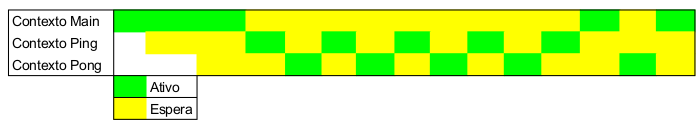
\includegraphics[width=\textwidth]{time_diagram.png}
	\caption{Diagrama de tempo da execução do código gerado pelo arquivo \emph{contexts.c}}
	\label{fig:tim_digr}
\end{figure}

É considerado que a criação e a configuração do contexto é feita de imediato. Por isso não foi adicionado um período de contexto ativo entre a criação o uso do \texttt{makecontext}.

\section{Conclusão}

Neste relatório foram apresentados conceitos relacionados a implementação de operações envolvendo contextos em ambiente UNIX. Além disso,  é explicado o funcionamento do exemplo de código presente no arquivo \emph{contexts.c} e feito o diagrama de tempo da execução.
% definição do estilo e inclusão da bibliografia
\bibliographystyle{plain}
\bibliography{referencias}

\end{document}

%=====================================================
